\documentclass[letter]{article}
\renewcommand{\baselinestretch}{1.25}

\usepackage[margin=1in]{geometry}
\usepackage{physics}
\usepackage{amsmath}
\usepackage{graphicx}
%\usepackage{pythonhighlight}
\usepackage{hyperref}
\usepackage{fancyvrb}

% MATLAB Formating Code
\usepackage[numbered,framed]{matlab-prettifier}
\lstset{style=Matlab-editor,columns=fullflexible}
\renewcommand{\lstlistingname}{Script}
\newcommand{\scriptname}{\lstlistingname}

% Command for easier minimization problem def
\newcommand{\optpblm}[3][eq:default]{
	\begin{equation}\label{#1}
% Array method... more centered		
%		\begin{array}{rl}
%			\text{minimize}  \hspace{0.2in} &#2 \vspace{5pt}\\
%			\text{subject to} \hspace{0.2in} &#3
%		\end{array}
% Aligned method... left aligned... idk if its better
		\begin{aligned}
			\text{minimize} \hspace{0.5in} &#2\vspace{5pt}\\
			\text{subject to \hspace{0.5in}} &#3
		\end{aligned}	
	\end{equation}
}

\newcommand{\maxpblm}[3][eq:default]{
	\begin{equation}\label{#1}
		\begin{aligned}
			\text{maximize} \hspace{0.5in} &#2\vspace{5pt}\\
			\text{subject to \hspace{0.5in}} &#3
		\end{aligned}	
	\end{equation}
}
\allowdisplaybreaks

\title{MECH 6327 - Homework 5}
\author{Jonas Wagner}
\date{2021, May 3}




\begin{document}

\maketitle

\tableofcontents

\newpage
\section{Control Design via SDP}
Consider the linearized model of a Cessna Citation Aircraft (at 5000m, at speed 128.2 m/s)
\begin{equation}
	\begin{aligned}
		\dot{x} &= \mqty[-1.2822 & 0 & 0.98 &0\\
						 0 & 0 &1 &0\\
						 -5.4293 &0 &-1.8366 &0\\
						 -128.2 &128.2 &0 &0] x
				+ \mqty[-0.3\\ 0\\ -17\\ 0] u
				+ \mqty[0\\ 0\\ 1\\0]w
		y		&= \mqty[0&1&0&0\\ 0&0&0&1\\ 0&0&0&0] x
				+ \mqty[0\\0\\1]u	
	\end{aligned}
\end{equation}
with control input $u$ = elevator angle, states $x_1$ = angle of at-
tack, $x_2$ = pitch angle, $x_3$ = pitch rate, and $x_4$ = altitude (all
relative to nominal), performance output $y$, and pitch rate disturbance input $w$.\\

\noindent
\textbf{Problem:}
Use the SDP formulations discussed in class to compute the optimal state feedback controller to minimize both the $\mathcal{H}_2$- and $\mathcal{H}_\infty$-norm from disturbance input $w$ to output $y$.
Also provide the optimal value for the respective closed-loop system norms.

\subsection{$\mathcal{H}_2$-norm}
The procedure outlined in class was implimented in CVX as seen in \appendixname \ \ref{apx:matlab_pblm1}, which resulted with the following results:
\begin{Verbatim}
K_H2 =

	-44.6546   56.8903    1.7838    1.0000


Norm_H2 =

	0.5000
\end{Verbatim}

\subsection{$\mathcal{H}_\infty$-norm}
The procedure outlined in class was implimented in CVX as seen in \appendixname \ \ref{apx:matlab_pblm1}, which resulted with the following results:
\begin{Verbatim}
K_Hinfty =

	1.0e+05 *

	-0.9457    1.1643    0.0299    0.0281


Norm_Hinfty =

	0.1330
\end{Verbatim}



\newpage
\section{Model Predictive Control (MPC)}
Suppose the elevator angle input is limited to $\pm0:262$rad ($\pm 15$ degrees), the elevator angle rate is limited to $\pm0:524$rad/s ($\pm 30$ degrees/s), and we would like to limit the pitch angle to $\pm 0.349$ rad ($\pm 20$ degrees). Consider the time discretized system with sampling period dt = 0:25s, and discrete-time dynamics matrices $A = e^{A_c \dd{t}}, B = \dd{t} B_c + \frac{1}{2} \dd{t} A_c B_c + \frac{1}{6} \dd{t}^2 A_c^2 B_c$, where $A_c$ and $B_c$ are the
above continuous time state space matrices.

\subsection{LQR Implementation}
\textbf{Problem:}
Compute the optimal infnite-horizon LQR controller by solving the discrete-time algebraic Riccati equation with $Q = I$ and $R = 10$.
Simulate the closed-loop system from initial state $x0 = \mqty[0 &0 &0 &10]^T$ but saturate the LQR controller to the input (magnitude and rate) constraints.\\

\noindent
\textbf{Solution:}
The calculation of an LQR controller gain was computed in MATLAB (\appendixname \ \ref{apx:matlab_pblm2}) and resulted in the following controller gain:
\begin{Verbatim}
K_LQR =
	
	2.6795   -3.6639   -0.1890   -0.0447
\end{Verbatim}

This was then simulated with the required saturation constraints as can be seen in \figurename \ \ref{fig:pblm2lqr}.

It is clear that the LQR controller had difficulty stabilizing the system given the saturation requirements on the elevator position and rate. It is not only clear that the control signal was saturated and limited by the maximum rate requirements, but that state $x_2$ is well outside of the desired bounds. (It is also just obvious that the system is unstable and will likely continue with increasing magnitudes periodic movements)


\begin{figure}[p]
	\centering
	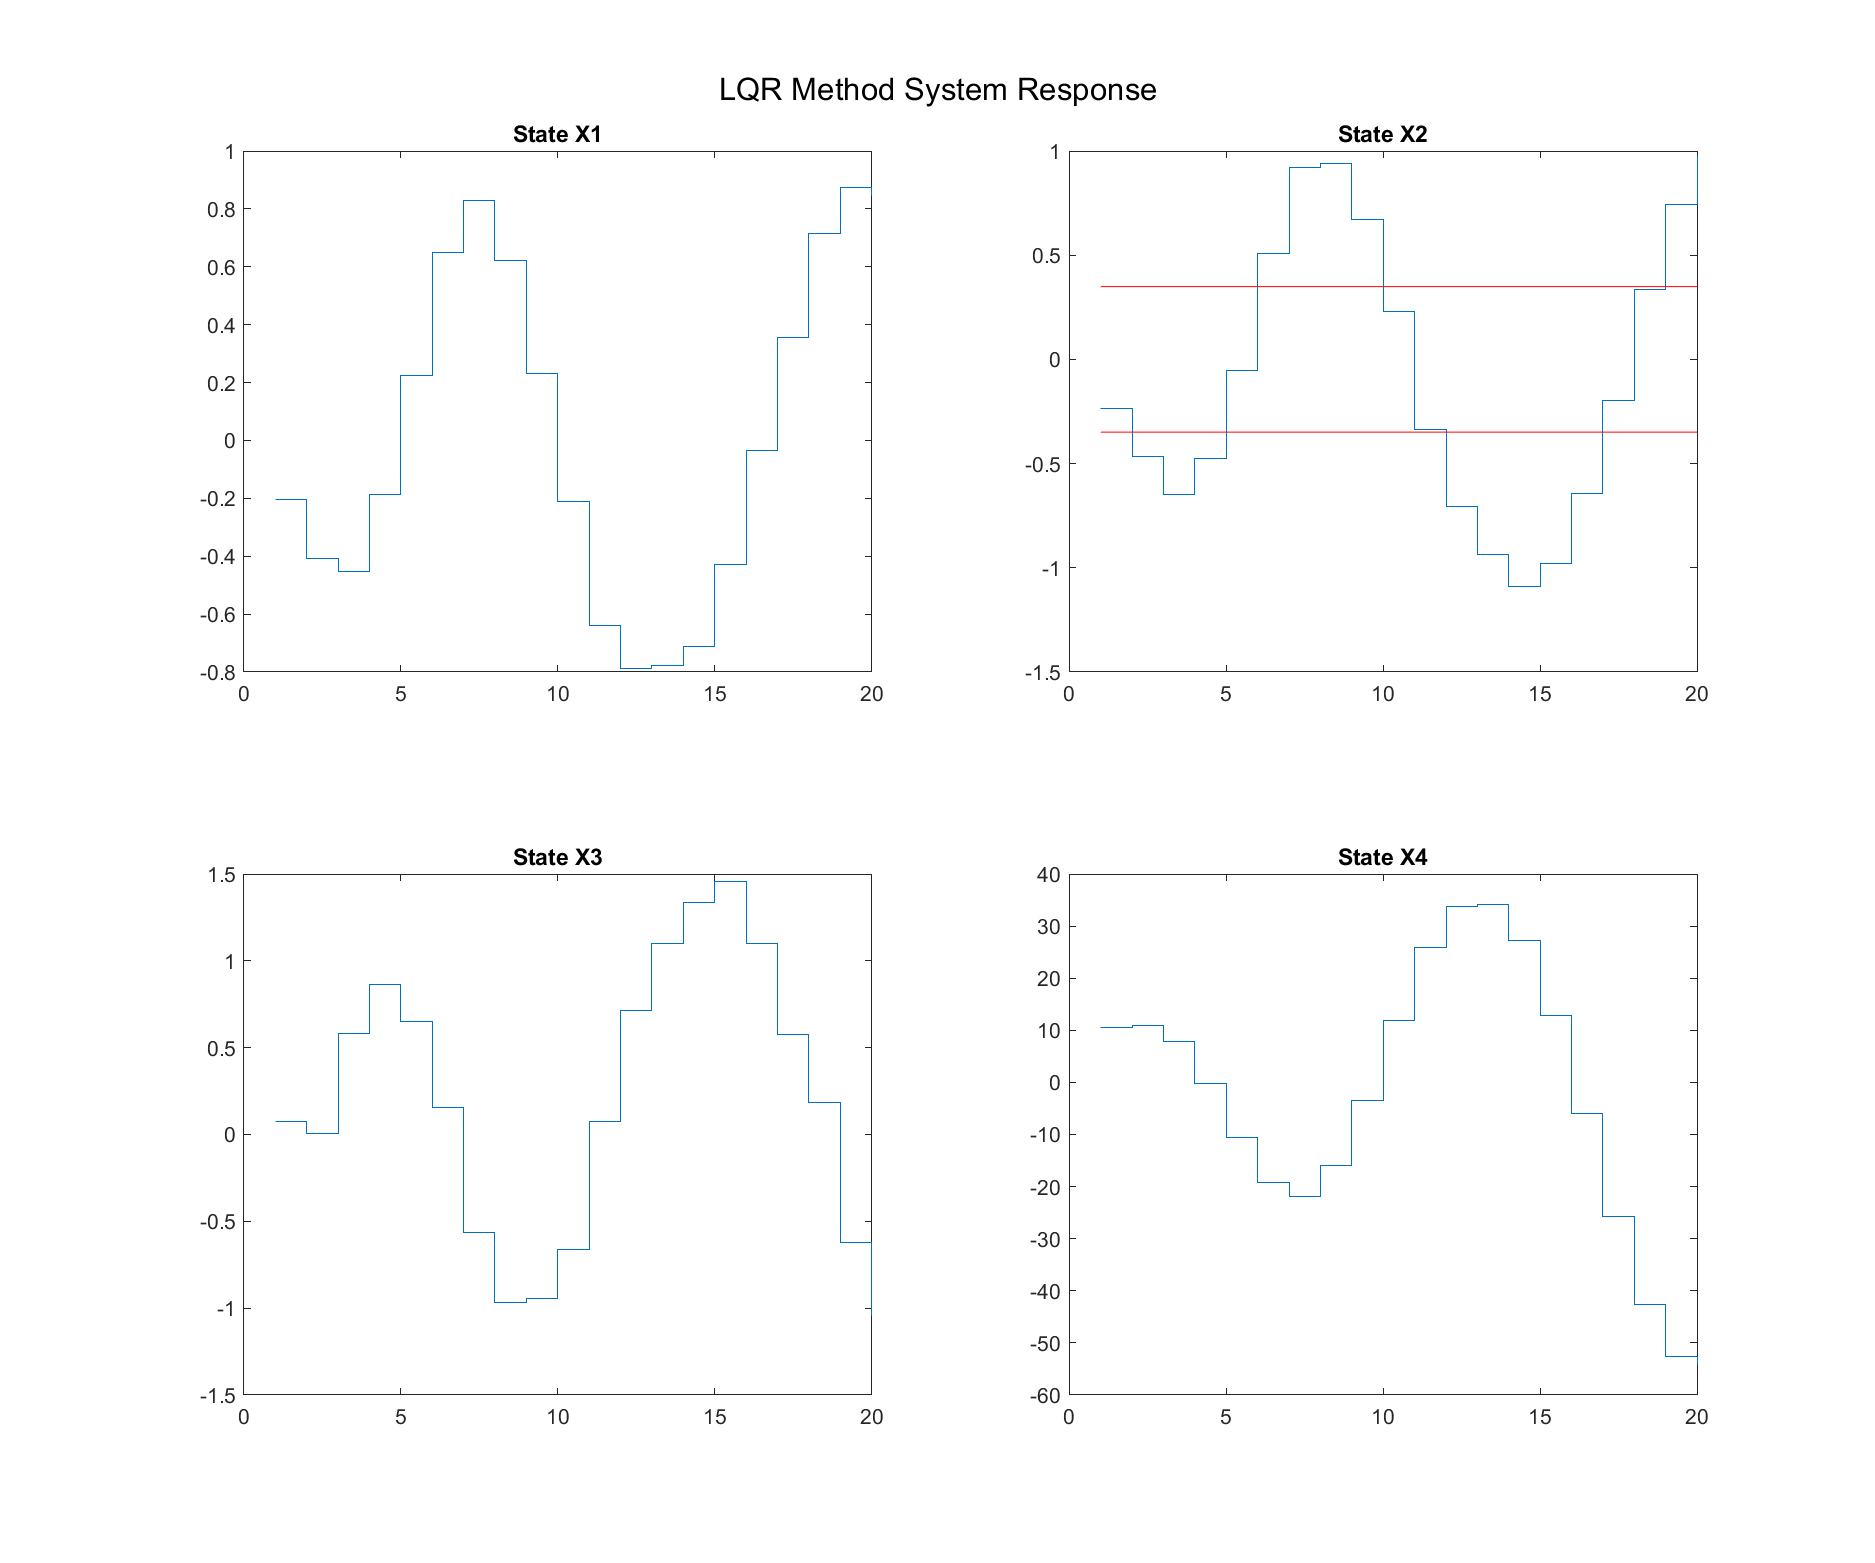
\includegraphics[width=\linewidth]{fig/pblm2_LQR_sys_response}
	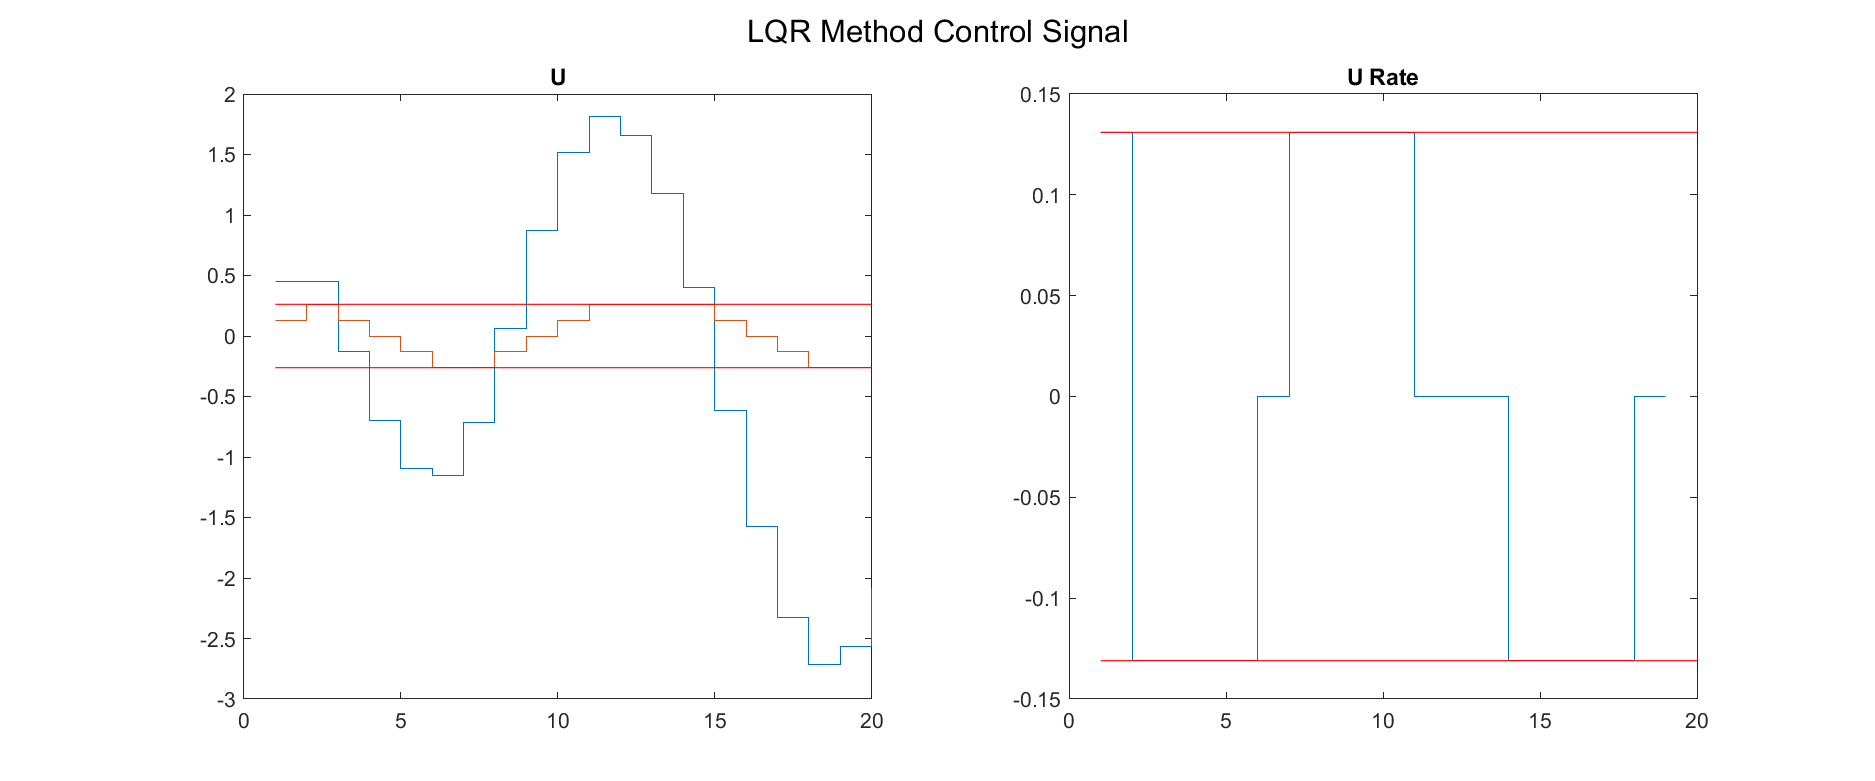
\includegraphics[width=\linewidth]{fig/pblm2_LQR_ctrl_signal}
	\caption{System response and control signal for the implementation of an infinite time LQR controller.}
	\label{fig:pblm2lqr}
\end{figure}


\newpage
\subsection{MPC Implementation}
\textbf{Problem:}
Implement a model predictive controller with horizon $T_h = 10$ sample periods and constant quadratic cost parameters $Q = I$ and $R = 10$ that explicitly accounts for the elevator angle and pitch constraints.
Simulate the closed-loop system from initial state $x0 = \mqty[0 &0 &0 &10]^T$ and compare to the LQR controller.
Determine using your implementation how short the MPC planning horizon can be reduced before stability problems arise.\\

\noindent
\textbf{Solution:}
The MPC was implimentated in MATLAB (\appendixname \ \ref{apx:matlab_pblm2}) and was then tested for multiple time horizons.

\subsubsection{$T_h = 10$}
In the original implementation (\figurename \ \ref{fig:pblm2mpcT10}), the controller is very effective (especially in comparison to the LQR controller). It is clear that the MPC implementation was able to intrinsically limit itself to the control limitations while also stabilizing the system effectively and within the desired timeframe while also staying within the ranges of $x_2$ dictated by the design goals.

\begin{figure}[p]
	\centering
	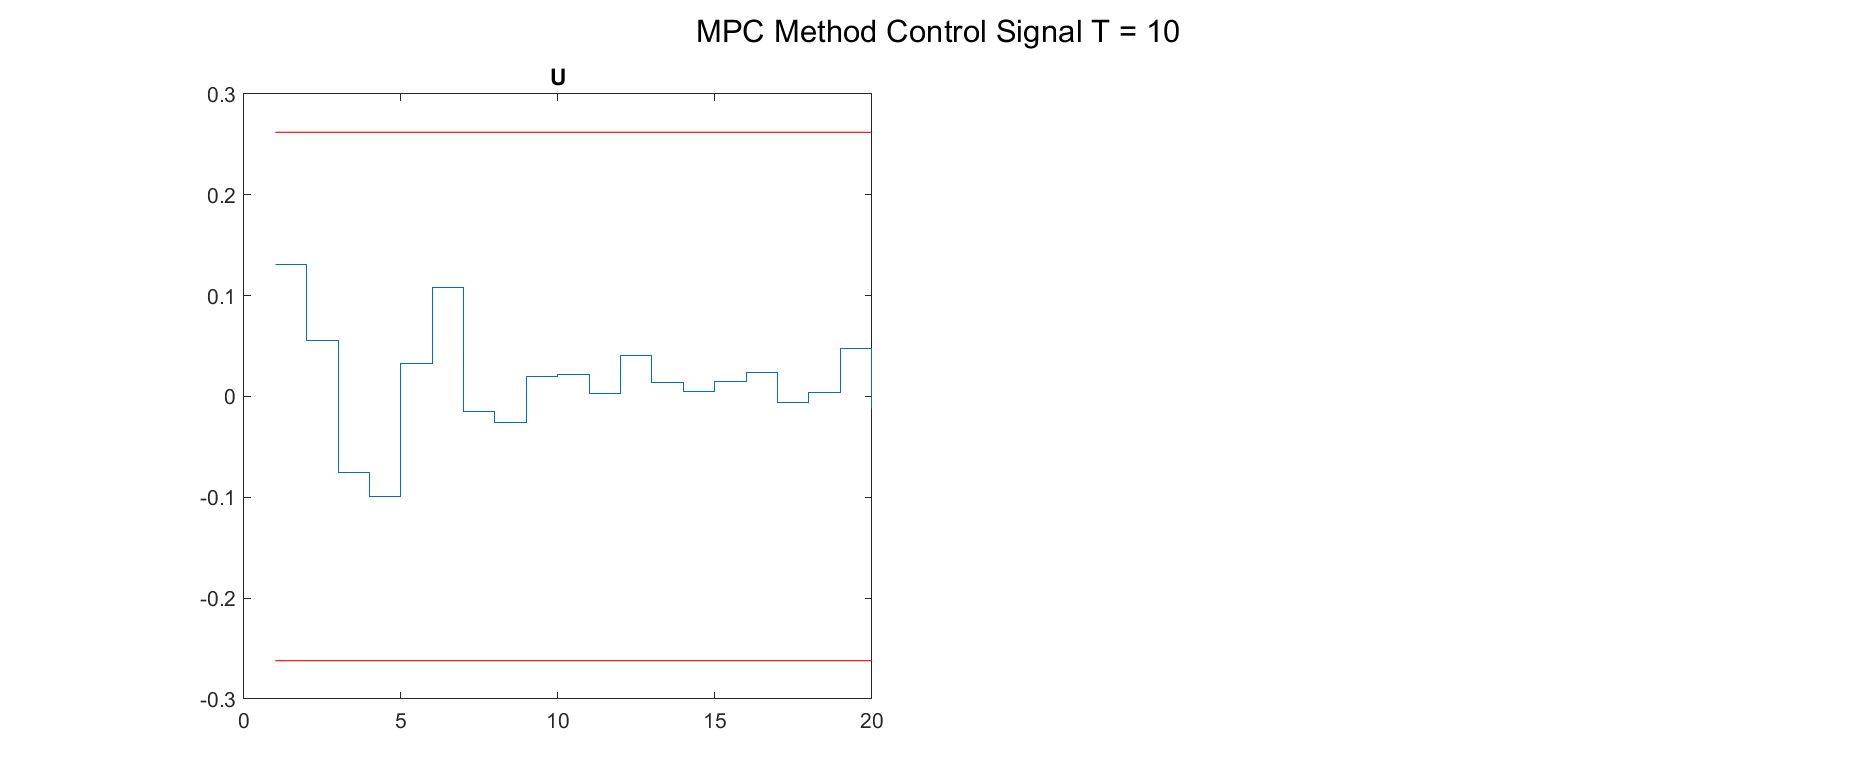
\includegraphics[width=\linewidth]{fig/pblm2_MPC_T10_sys_response}
	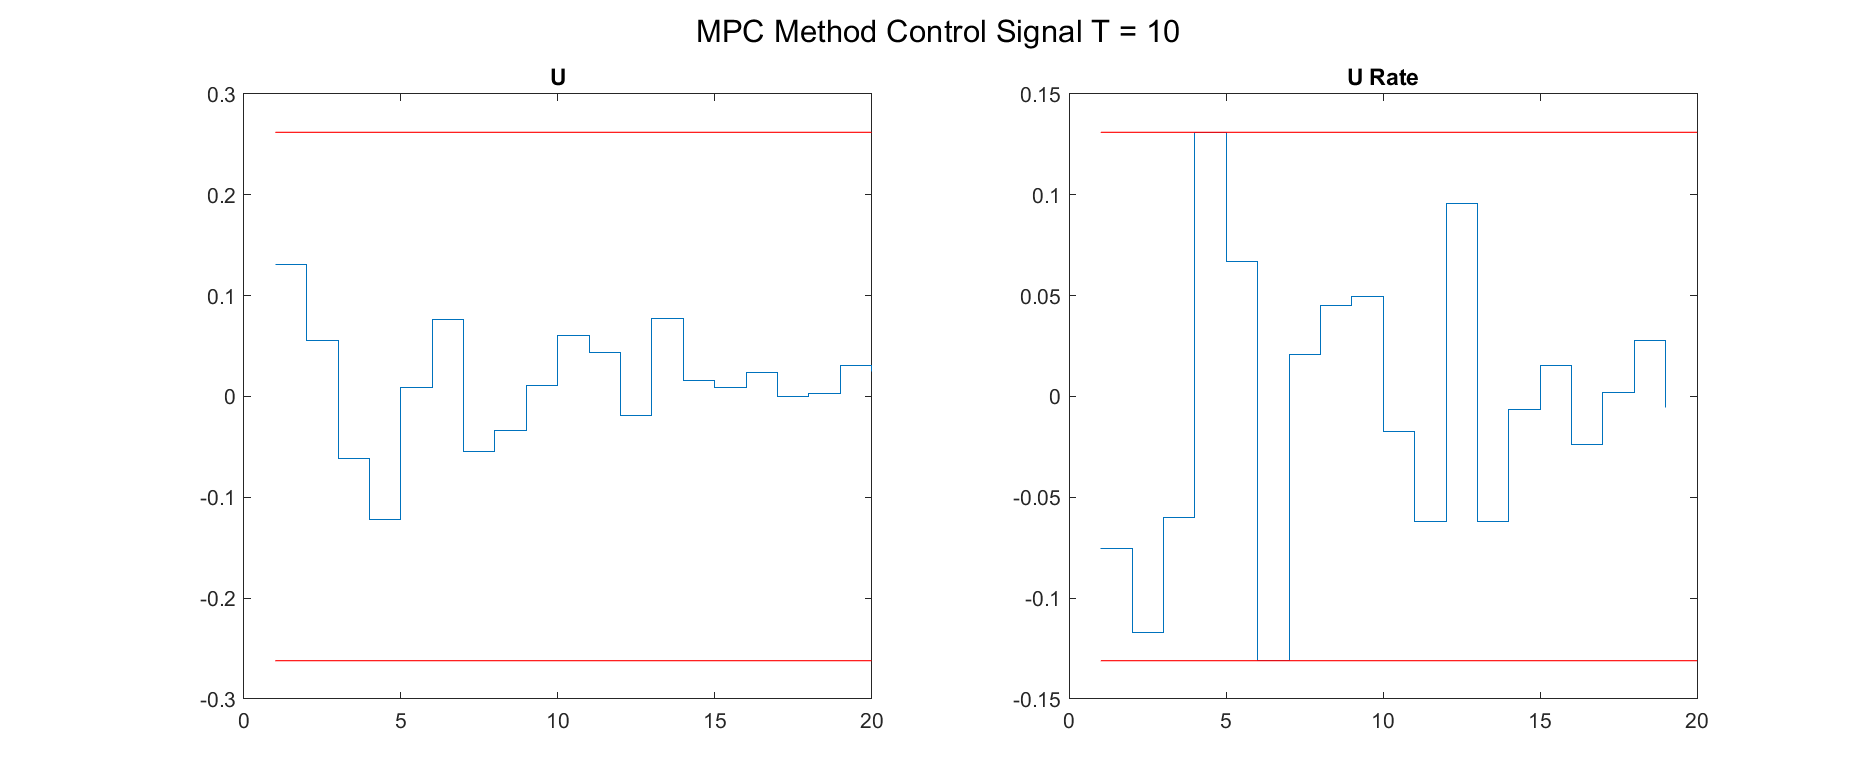
\includegraphics[width=\linewidth]{fig/pblm2_MPC_T10_ctrl_signal}
	\caption{System response and control signal for the implementation of an MPC with $T_h = 10$.}
	\label{fig:pblm2mpcT10}
\end{figure}

\subsubsection{$T_h = 5$}
The MPC implementation for $T_h = 5$ (\figurename \ \ref{fig:pblm2mpcT5}) was also effective. Compared to the longer time-horizon implementations, the system appears to have slightly larger control-signal magnitudes as well as a faster, yet more volatile, response for the individual state responses.

\begin{figure}[p]
	\centering
	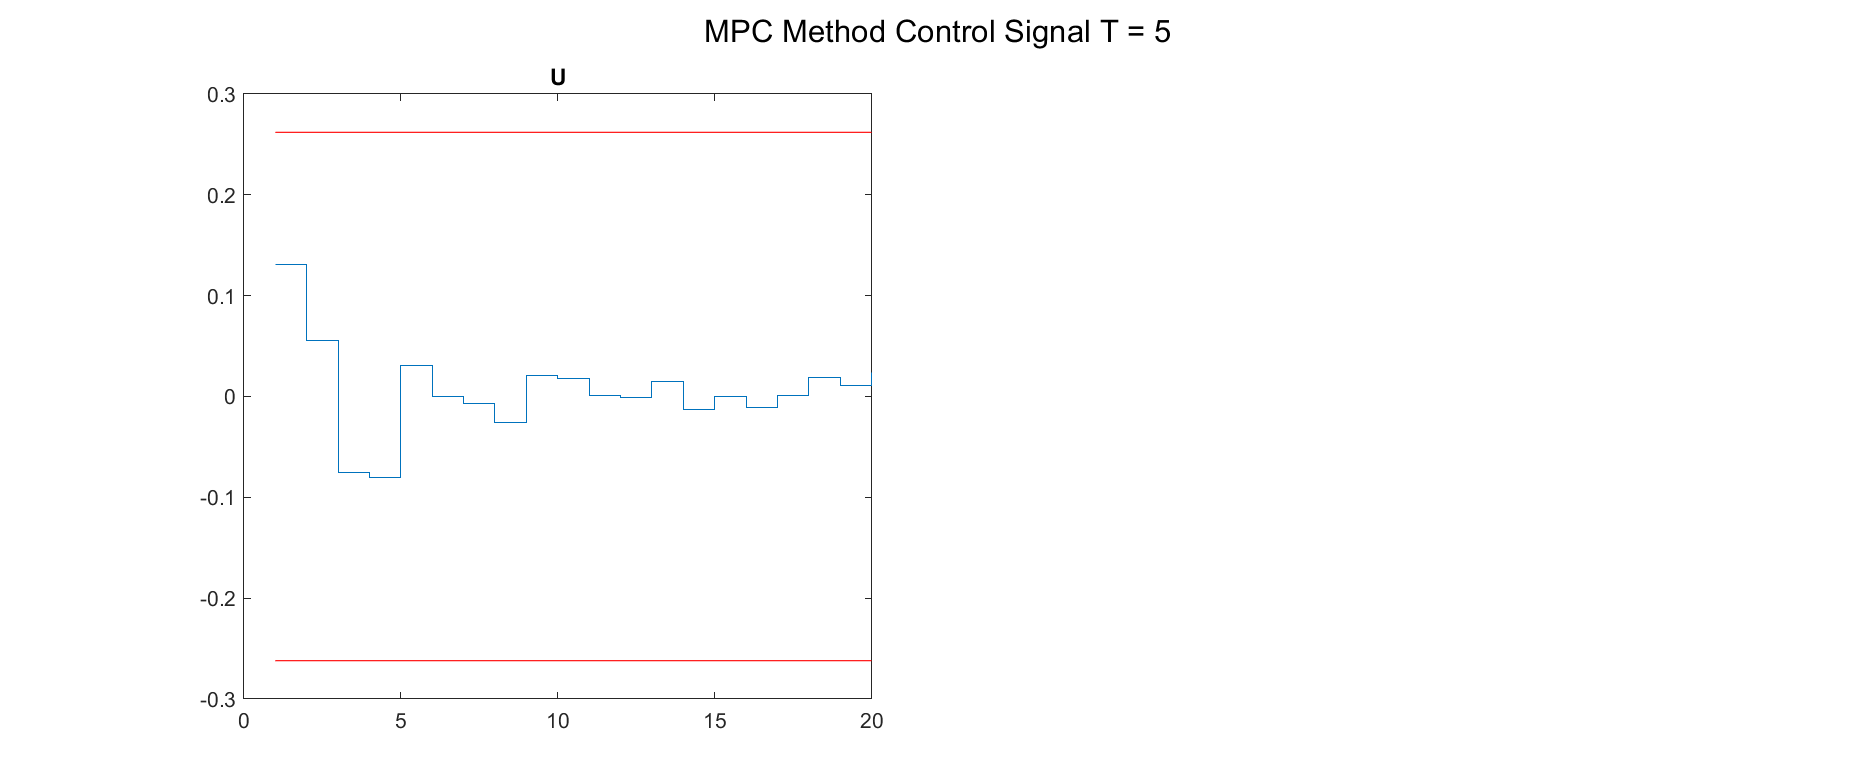
\includegraphics[width=\linewidth]{fig/pblm2_MPC_T5_sys_response}
	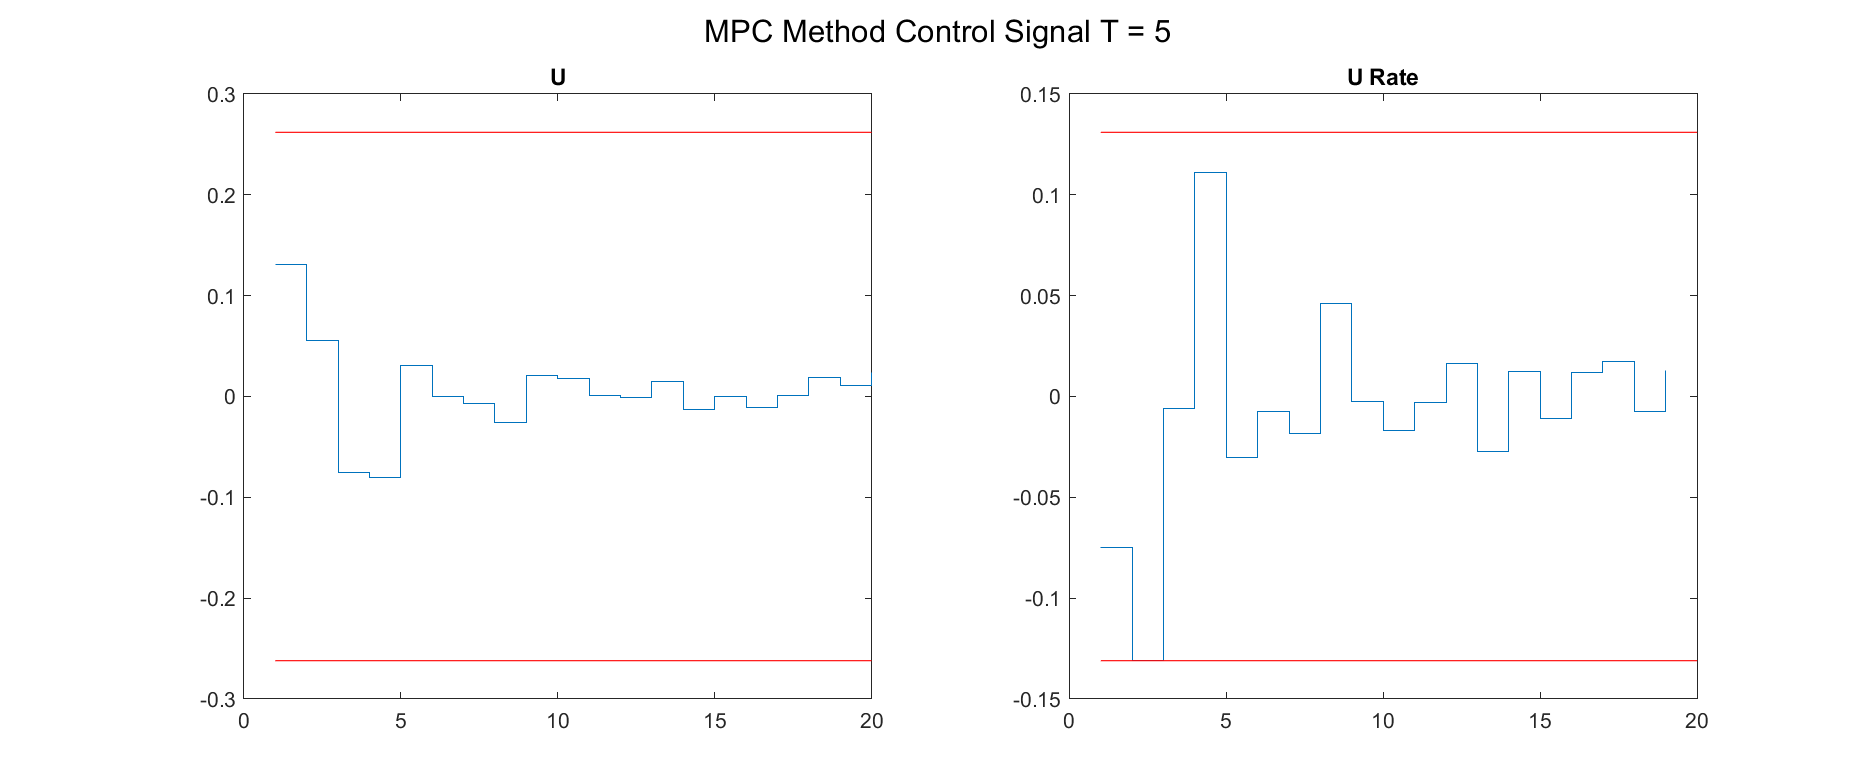
\includegraphics[width=\linewidth]{fig/pblm2_MPC_T5_ctrl_signal}
	\caption{System response and control signal for the implementation of an MPC with $T_h = 5$.}
	\label{fig:pblm2mpcT5}
\end{figure}

\subsubsection{$T-h = 3$}
The MPC implementation for $T_h = 3$ (\figurename \ \ref{fig:pblm2mpcT3}) the system no longer stabalizable. Compared to the longer time-horizon implementations, the system has a troublesome appearance of uncontrolled ossilations that untimely cause state $x_2$ to reach outside of the desired bounds.

\begin{figure}[p]
	\centering
	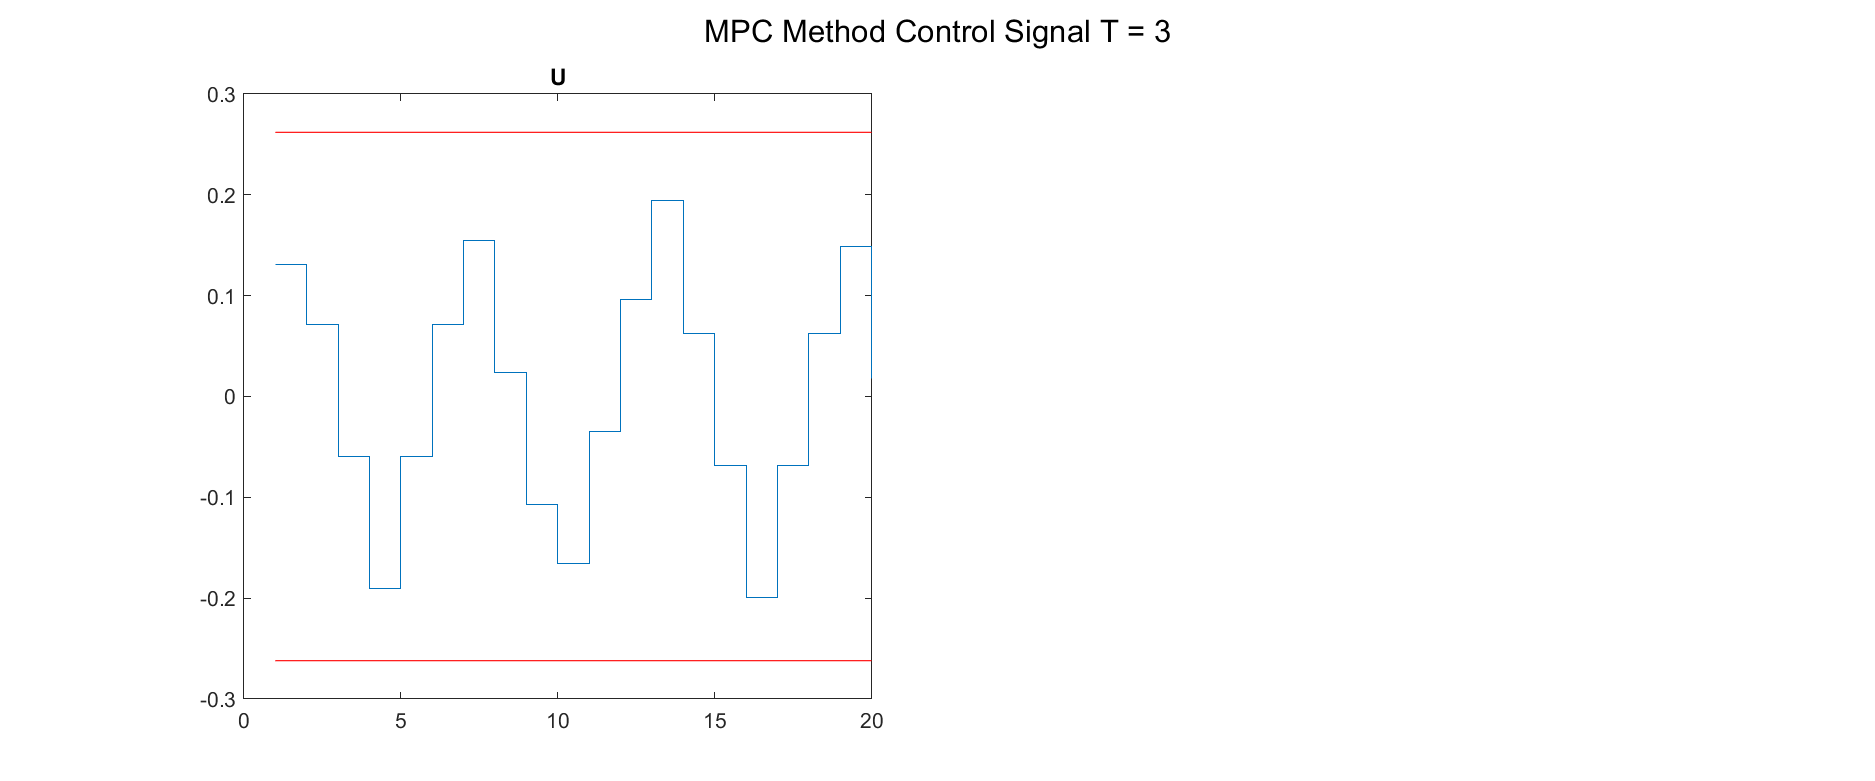
\includegraphics[width=\linewidth]{fig/pblm2_MPC_T3_sys_response}
	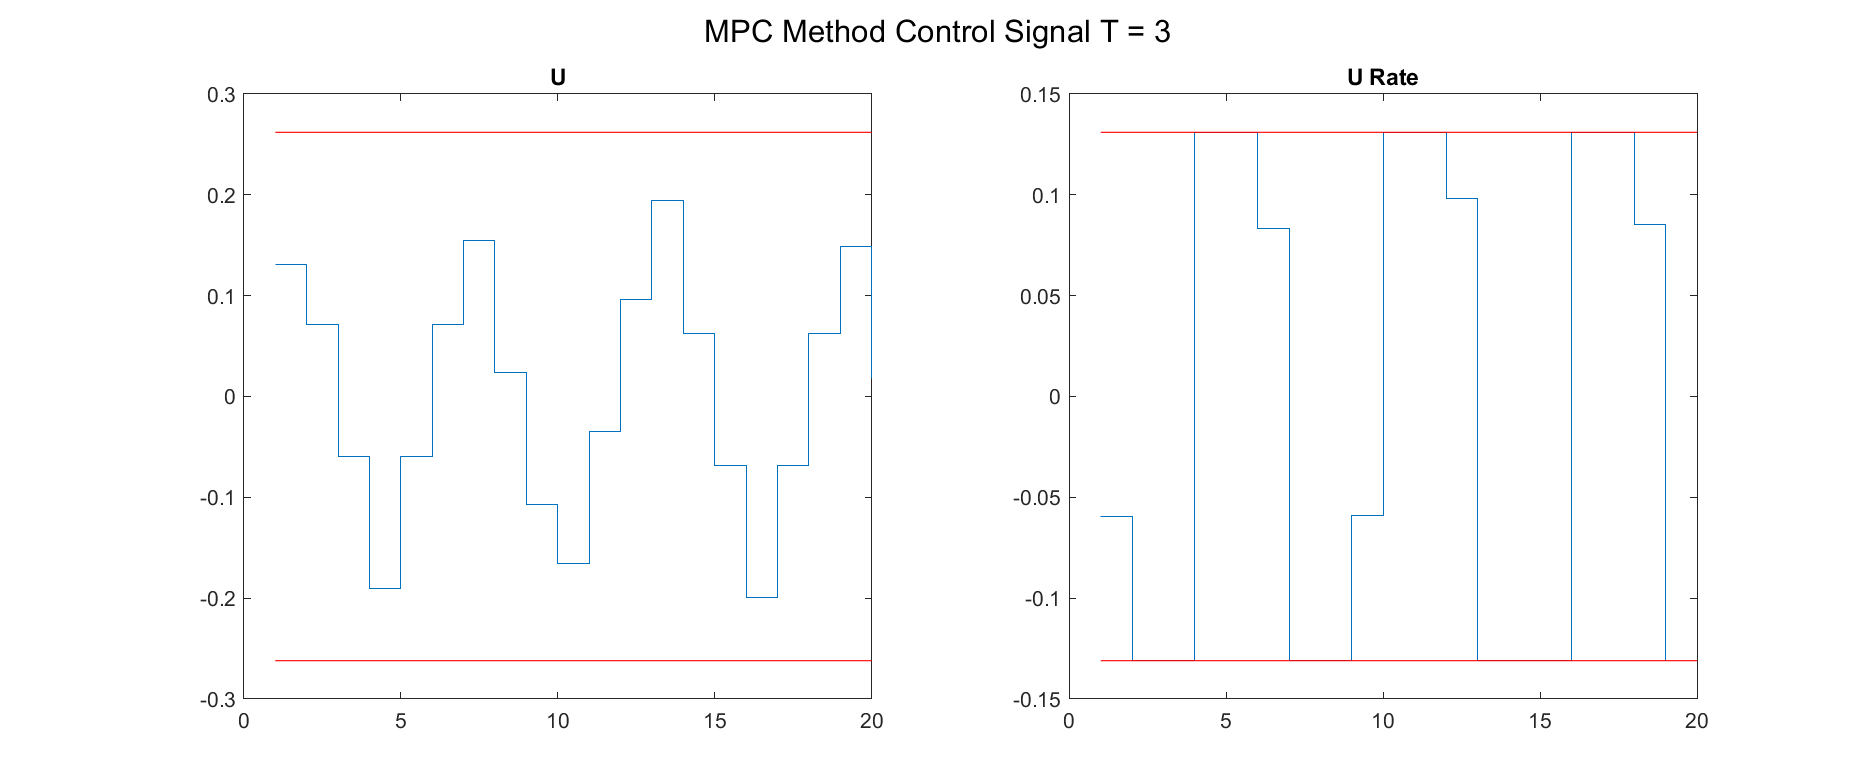
\includegraphics[width=\linewidth]{fig/pblm2_MPC_T3_ctrl_signal}
	\caption{System response and control signal for the implementation of an MPC with $T_h = 3$.}
	\label{fig:pblm2mpcT3}
\end{figure}

\subsubsection{$T-h = 20$}
A very different result occurs when the time-horizon is increased, as opposed to decreased. The MPC implementation for $T_h = 20$ (\figurename \ \ref{fig:pblm2mpcT20}) is even more effective then the original $T_h = 10$ implementation. All of the states quickly stabalized and are then maintained with very little control effort.

\begin{figure}[p]
	\centering
	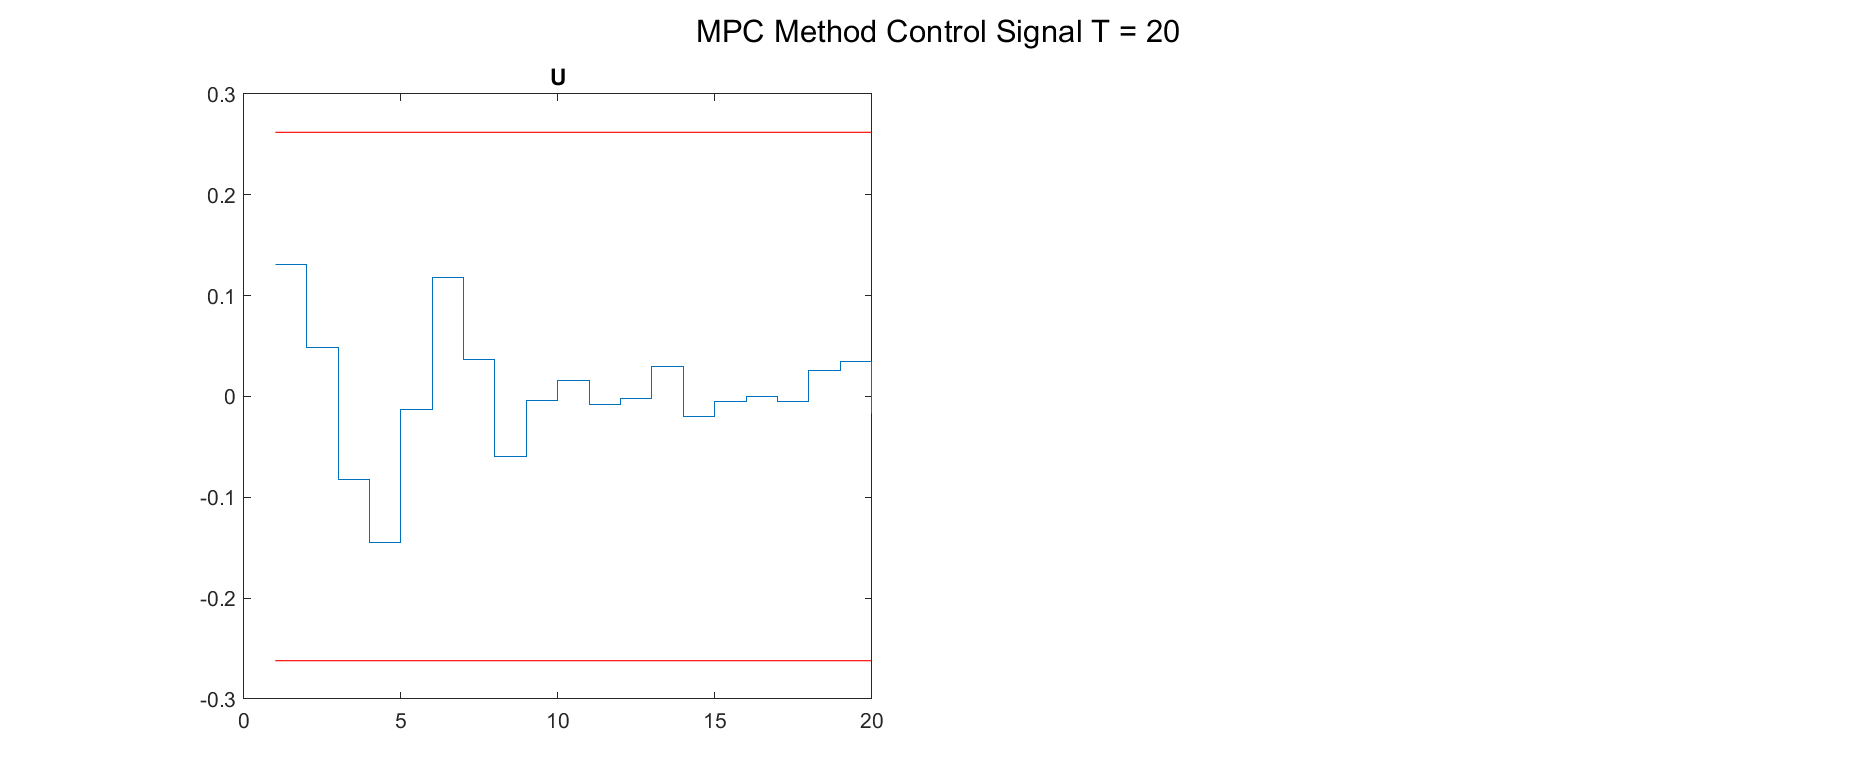
\includegraphics[width=\linewidth]{fig/pblm2_MPC_T20_sys_response}
	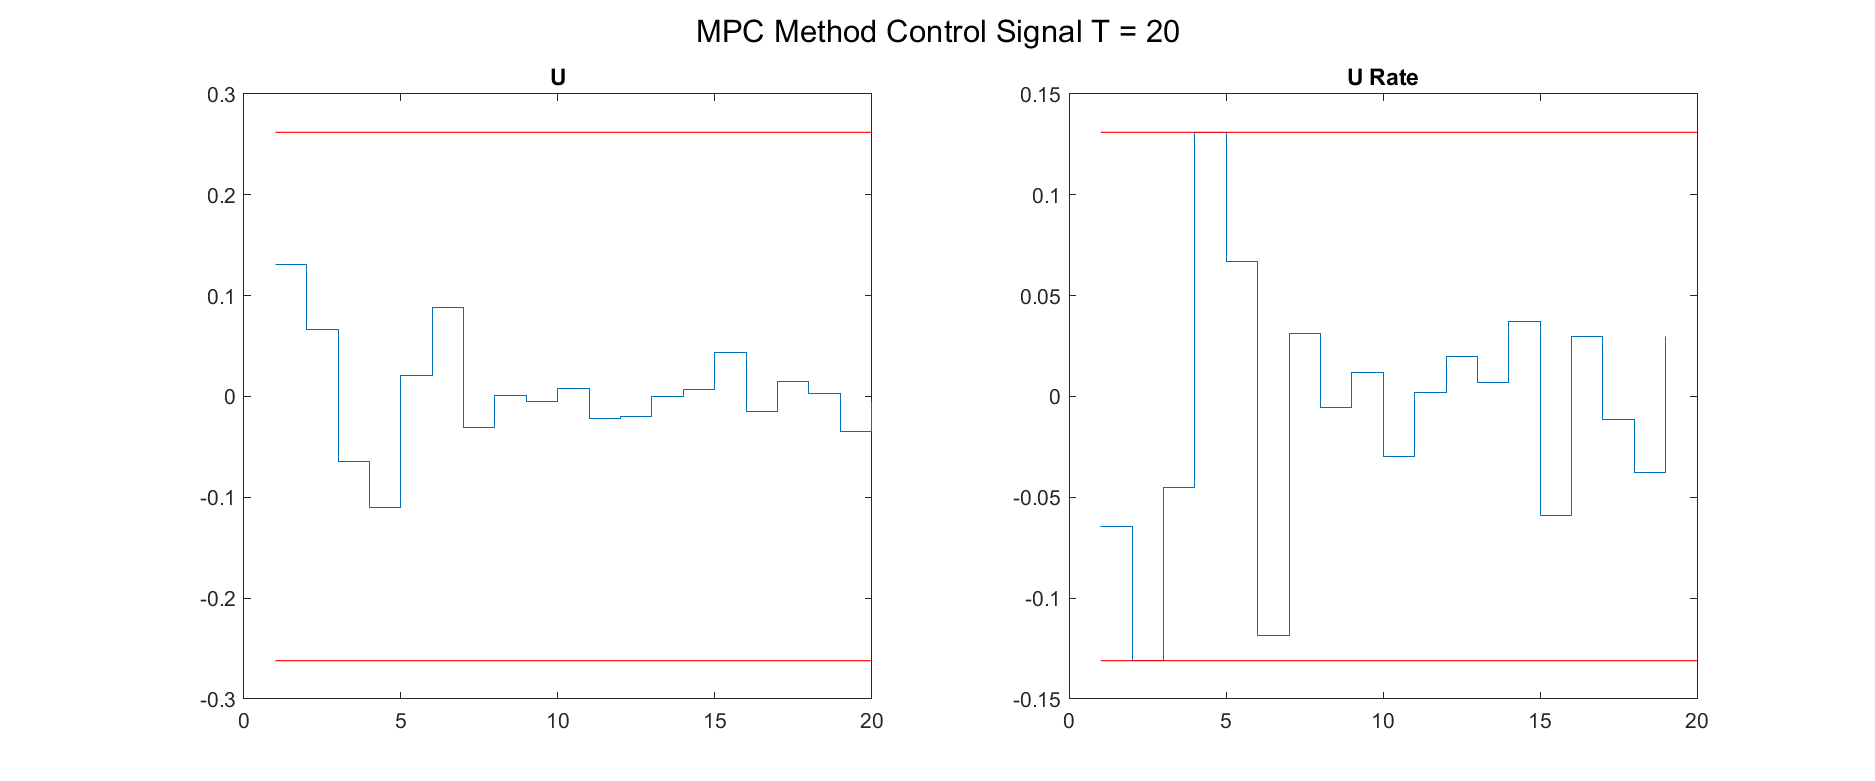
\includegraphics[width=\linewidth]{fig/pblm2_MPC_T20_ctrl_signal}
	\caption{System response and control signal for the implementation of an MPC with $T_h = 20$.}
	\label{fig:pblm2mpcT20}
\end{figure}




\newpage
\appendix
\section{MATLAB Code:}\label{apx:matlab}
All code I write in this course can be found on my GitHub repository:\\
\href{https://github.com/jonaswagner2826/MECH6337}{https://github.com/jonaswagner2826/MECH6327}
\lstinputlisting[caption={MECH6327\_HW5},label={script:HW5}]{MECH6327_HW5.m}
\newpage
\subsection{Problem 1 Code}\label{apx:matlab_pblm1}
\lstinputlisting[caption={MECH6327\_HW5\_pblm1},label={script:HW5_pblm1}]{MECH6327_HW5_pblm1.m}
\newpage
\subsection{Problem 2 Code}\label{apx:matlab_pblm2}
\lstinputlisting[caption={MECH6327\_HW5\_pblm2},label={script:HW5_pblm2}]{MECH6327_HW5_pblm2.m}


\end{document}